%-------------------------------------------------------
% HEADER
%-------------------------------------------------------

\documentclass[10pt, aspectratio=169]{beamer}
\usetheme[]{Feather}
 %Change the bar colors:
%\setbeamercolor{Feather}{fg=green!20,bg=green}
% Change the color of the structural elements:
%\setbeamercolor{structure}{fg=red}
% Change the frame title text color:
%\setbeamercolor{frametitle}{fg=blue}
% Change the normal text color background:
%\setbeamercolor{normal text}{fg=black,bg=gray!10}
\usepackage[utf8]{inputenc} %default packages
\usepackage[english]{babel}
\usepackage[T1]{fontenc}
\usepackage[scaled]{helvet}
\usefonttheme[onlymath]{serif} %For LaTeX-style looking equations
\usepackage{amsfonts} %default packages
\usepackage{amsmath}
\usepackage{amssymb}
\usepackage{amsthm}
\usepackage{amstext}
\usepackage{tikz} %making graphs within LaTeX
\usepackage{graphicx}
\usepackage{mathtools} %drawing picture with tikz
\usepackage{pgfplots} %making plots within LaTeX
\usepackage{pgfplotstable} %for importing data from csv files
\pgfplotsset{compat=1.17}
\usepackage{tabularx} %for tables centered
\usepackage{booktabs} %for better looking tables
\usepackage{longtable}
\usepackage{subcaption} % provides subfigures within figures 
\usepackage[absolute,overlay]{textpos} %for placing figures wherever
\usepackage{animate} %for making GIF animations
%small font size for the bibliography at the end
\newcommand\Fontvi{\fontsize{6}{7.2}\selectfont}
\usepackage{float} % Package to place figures where you want them.

\newcommand{\tagg}[1]{%
	\tikz[baseline]\node[anchor=base,
	draw=gray!30,
	rounded corners,
	inner xsep=1ex,
	inner ysep =0.75ex,
	text height=1.5ex,
	text depth=.25ex]{#1};
  }


%pgfplots style list (color and style of the plots for each farmer)
\definecolor{farmer1}{HTML}{f28d11} %orange
\definecolor{farmer2}{HTML}{0e5de8} %blue
\definecolor{farmer3}{HTML}{2bd941} %green
\definecolor{farmer4}{HTML}{d41717} %red
\definecolor{crop1}{HTML}{e41a1c} %
\definecolor{crop2}{HTML}{377eb8} %
\definecolor{crop3}{HTML}{4daf4a} %
\definecolor{crop4}{HTML}{984ea3} %
\pgfplotscreateplotcyclelist{farmerslist}{
%Farmer 1
farmer1,every mark/.append style={farmer1},mark=triangle*\\
%Farmer 2
farmer2,every mark/.append style={farmer2},mark=diamond*\\
%Farmer 3
farmer3,every mark/.append style={farmer3},mark=otimes\\
%Farmer 4
farmer4,every mark/.append style={farmer4},mark=star\\
%etc...
}
\pgfplotscreateplotcyclelist{cropslist}{
crop1, thick, every mark/.append style={crop1}, mark=triangle\\
crop2,every mark/.append style={crop2},mark=diamond\\
crop3,every mark/.append style={crop3},mark=otimes\\
crop4, densely dashed,every mark/.append style={crop4},mark=square*\\
%etc...
}


%-------------------------------------------------------
% INFORMATION IN THE TITLE PAGE
%-------------------------------------------------------

\title[] % [] is optional - is placed on the bottom of the sidebar on every slide
{ % is placed on the title page
      \textbf{851-0101-86 S Complex Social Systems: Modeling Agents, Learning, and Games}
}

\subtitle[]
{
      \textbf{CropWar: Agent-based simulation of agricultural interactions}
}

\author[]
{      C.Golling, G.Mourouga, A.Moser, O.Schmidt, A.H.Keshavarzzadeh
      {}
}

\institute[]
{
      %GDR redox-flow
  
  %there must be an empty line above this line - otherwise some unwanted space is added between the university and the country (I do not know why;( )
}

\date{}

%Programatically defining the sections to be called on the slides title
\def\z{Introduction and motivation}
\def\a{The CropWar model}
\def\aa{Deterministic versions}
\def\aaa{Basic version: selling and stocking}
\def\aab{The Map class: expansion}
\def\aac{The Market model: dynamic pricing}
\def\aad{Agent personalities}
\def\aae{Weather events}
\def\ab{Reinforcement Learning versions}
\def\aba{Tianshu basics}
\def\abb{Tests with different personalities}

\def\b{Summary and Outlook}

%-------------------------------------------------------
% START OF DOCUMENT
%-------------------------------------------------------

\begin{document}

%-------------------------------------------------------
% THE TITLEPAGE
%-------------------------------------------------------

{\1% % this is the name of the PDF file for the background
\begin{frame}[plain,noframenumbering] % the plain option removes the header from the title page, noframenumbering removes the numbering of this frame only
  \titlepage % call the title page information from above
\end{frame}}


\begin{frame}{Content}{}
    \tableofcontents
\end{frame}

%-------------------------------------------------------
\section{\z}
%-------------------------------------------------------

\begin{frame}{\z}
  \onslide<1->{\texttt{CropWar} aims at modelling \textbf{interactions between farmers} growing crops in a \textbf{geographic area} with a finite amount of \textbf{water ressources} and selling them on a \textbf{market} to feed a population.}\\
 \onslide<2->{The model is organised as follows:}
 \begin{itemize}
  \item<3-> \tagg{v1.1} basic version: growing, selling, stocking
  \item<4-> \tagg{v1.2} implementation of the \texttt{Map} class: spatial expansion
  \item<5-> \tagg{v1.3} implementation of the \texttt{Market} model: dynamic pricing
  \item<6-> \tagg{v1.4} implementation of agent personalities: game theory
  \item<7-> \tagg{v2.1} reinforcement learning: identifying the optimal strategy
\end{itemize}
\end{frame}

%-------------------------------------------------------
\section{\z}
%-------------------------------------------------------

\subsection{\aa}
%-------------------------------------------------------

\subsubsection{\aaa}
\begin{frame}{\aa}{\aaa}
  \centering
  \textbf{v1.1: Basic version}
\end{frame}


\begin{frame}{\aa}{\aaa}
    \begin{columns}
      \column{0.48\linewidth}
         \centering
         \begin{figure}
          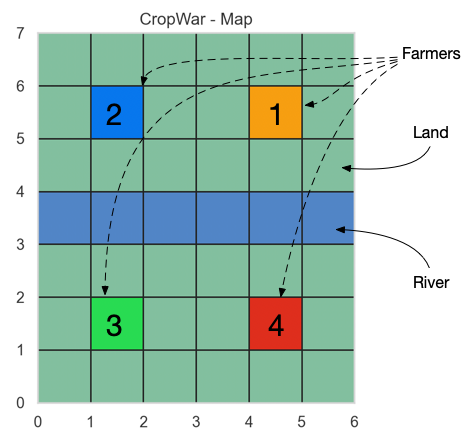
\includegraphics[width=\textwidth]{Figures/v11_Map.png}
         \end{figure}
       \column{0.52\linewidth}
       In \tagg{v1.1} farmers only have access to one cell on which they can choose to grow one of two crops (A or B)
     \end{columns} 
\end{frame}

\pgfplotstableread[col sep=comma]{Data/v11_exported_budget.csv}{\budgeta}
\pgfplotstableread[col sep=comma, skip first n=3]{Data/v11_exported_stock.csv}{\stocka}

\begin{frame}{\aa}{\aaa}
  \begin{columns}
    \column{0.48\linewidth}
       \centering
       \begin{figure}
       \resizebox{\linewidth}{!}{\begin{tikzpicture}
  \pgfplotsset{
    scale only axis,
  }
  %axis options:
  \begin{axis}[
    xlabel=Time step (years),
    ylabel=Farmer stock,
    xmin=0,
    %ymin=350,
    legend pos=north west,
    cycle list name=farmerslist
  ]
    %plot 1: farmer ID 1
    \addplot+[] table[y index =1]{\stocka};
    \addlegendentry{$1$}
    
    %plot 2: farmer ID 2
    \addplot+[]  table[y index =2]{\stocka};
    \addlegendentry{$2$}

    %plot 3: farmer ID 3
    \addplot+[dashed] table[y index =7]{\stocka};
    \addlegendentry{$3$}

    %plot 4: farmer ID 4
    \addplot+[] table[y index =4]{\stocka};
    \addlegendentry{$4$}

  \end{axis}
  \end{tikzpicture}
  }
       \end{figure}
     \column{0.52\linewidth}
     This plot shows the evolution of stock as a function of time:\\
     Farmers 1,2 and 4 grow crop A\\
     Farmer 3 grows crop B\\
     At each time step, they chose to stock or sell their yield
   \end{columns} 
\end{frame}

\begin{frame}{\aa}{\aaa}
    \begin{columns}
      \column{0.48\linewidth}
         \centering
         \begin{figure}
         \resizebox{\linewidth}{!}{\begin{tikzpicture}
		\pgfplotsset{
			scale only axis,
		}
		%axis options:
		\begin{axis}[
		  xlabel=Time step (years),
		  ylabel=Farmer wealth (\$),
		  xmin=0,
		  %ymin=350,
		  legend pos=north west,
		  cycle list name=farmerslist
		]
		  %plot 1: farmer ID 1
		  \addplot+[] table[y index =1]{\budgeta};
		  \addlegendentry{$1$}
		  
		  %plot 2: farmer ID 2
		  \addplot+[]  table[y index =2]{\budgeta};
		  \addlegendentry{$2$}
  
		  %plot 3: farmer ID 3
		  \addplot+[] table[y index =3]{\budgeta};
		  \addlegendentry{$3$}
  
		  %plot 4: farmer ID 4
		  \addplot+[] table[y index =4]{\budgeta};
		  \addlegendentry{$4$}
  
		\end{axis}
	  \end{tikzpicture}
	  }
         \end{figure}
       \column{0.52\linewidth}
       This plot shows the corresponding evolution of the farmer's wealth as a function of time.\\
       Selling corresponds to an increase in wealth, stocking to a constant value.
     \end{columns} 
\end{frame}

\subsubsection{\aab}

\begin{frame}{\aa}{\aab}
  \centering
  \textbf{v1.2: Spatial expansion}
\end{frame}

\begin{frame}{\aa}{\aab}
  \begin{columns}
    \column{0.48\linewidth}
    \centering
    \begin{figure}
      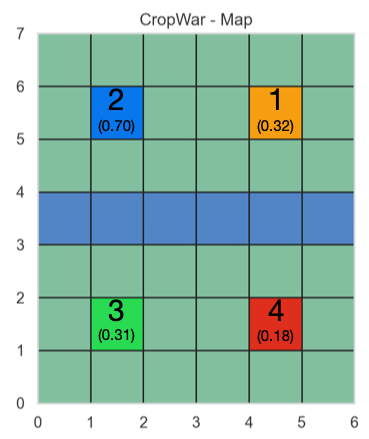
\includegraphics[width=.8\textwidth]{Figures/v12_Map_start.png}
     \end{figure}
    \column{0.52\linewidth}
     The \texttt{buy\_threshold} (in brackets) indicates the tendancy of farmers to expand their farms by buying neighbouring land in order to grow more crops
  \end{columns}
\end{frame}

\begin{frame}{\aa}{\aab}
  \begin{columns}
    \column{0.48\linewidth}
    \centering
    \begin{figure}
      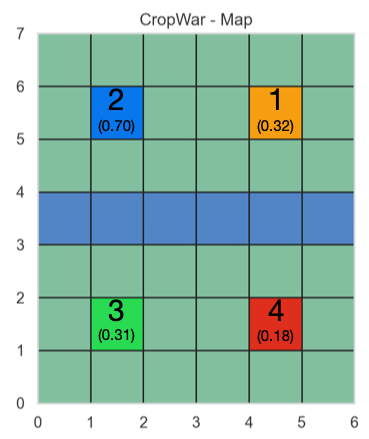
\includegraphics[width=.8\textwidth]{Figures/v12_Map_start.png}
     \end{figure}
    \column{0.52\linewidth}
    \centering
    \animategraphics[loop,width=5.8cm]{1}{Figures/V12mapGIF/frame_}{00}{10}
  \end{columns}
\end{frame}

\pgfplotstableread[col sep=comma]{Data/v12_exported_budget.csv}{\budgetb}
\pgfplotstableread[col sep=comma, skip first n=3]{Data/v12_exported_stock.csv}{\stockb}
\pgfplotstableread[col sep=comma, skip first n=1]{Data/v12_exported_cellcount.csv}{\cellcountb}

\begin{frame}{\aa}{\aab}
  \begin{columns}
    \column{0.48\linewidth}
    \resizebox{\linewidth}{!}{\begin{tikzpicture}
      \pgfplotsset{
        scale only axis,
      }
      %axis options:
      \begin{axis}[
        xlabel=Time step (years),
        ylabel=Farmer land count (cells),
        xmin=0,
        legend pos=north west,
        cycle list name=farmerslist
      ]
        %plot 1: farmer ID 1
        \addplot+[] 
          table[y index =1]{\cellcountb};
        \addlegendentry{$1$}
        
        %plot 2: farmer ID 2
        \addplot+[]  table[y index =2]{\cellcountb};
        \addlegendentry{$2$}
    
        %plot 3: farmer ID 3
        \addplot+[] table[y index =3]{\cellcountb};
        \addlegendentry{$3$}
    
        %plot 4: farmer ID 4
        \addplot+[] table[y index =4]{\cellcountb};
        \addlegendentry{$4$}
    
      \end{axis}
      \end{tikzpicture}
    }
    \column{0.52\linewidth}
    \resizebox{\linewidth}{!}{\begin{tikzpicture}
      \pgfplotsset{
        scale only axis,
      }
      
      \begin{axis}[
        xlabel=Time step (years),
        ylabel=Farmer stock,
        xmin=0,
        ymin=0,
        legend pos=north west,
        cycle list name=farmerslist
      ]
        %plot 1: farmer ID 1
      \addplot+[dashed] table[y index =5]{\stockb};
      \addlegendentry{$1$}
      
      %plot 2: farmer ID 2
      \addplot+[]  table[y index =2]{\stockb};
      \addlegendentry{$2$}
  
      %plot 3: farmer ID 3
      \addplot+[] table[y index =3]{\stockb};
      \addlegendentry{$3$}
  
      %plot 4: farmer ID 4
      \addplot+[] table[y index =4]{\stockb};
      \addlegendentry{$4$}
  
      \end{axis}
      \end{tikzpicture}
    }
  \end{columns}
\end{frame}

\begin{frame}{\aa}{\aab}
  \begin{columns}
    \column{0.48\linewidth}
    \centering
    \begin{figure}
      \resizebox{\linewidth}{!}{\begin{tikzpicture}
        \pgfplotsset{
          scale only axis,
        }
        %axis options:
        \begin{axis}[
          xlabel=Time step (years),
          ylabel=Farmer wealth (\$),
          xmin=0,
          ymax = 600,
          legend pos=north west,
          cycle list name=farmerslist
        ]
          %plot 1: farmer ID 1
          \addplot+[] 
            table[y index =1]{\budgetb};
          \addlegendentry{$1$}
          
          %plot 2: farmer ID 2
          \addplot+[]  table[y index =2]{\budgetb};
          \addlegendentry{$2$}
      
          %plot 3: farmer ID 3
          \addplot+[] table[y index =3]{\budgetb};
          \addlegendentry{$3$}
      
          %plot 4: farmer ID 4
          \addplot+[] table[y index =4]{\budgetb};
          \addlegendentry{$4$}
      
        \end{axis}
        \end{tikzpicture}
        }
     \end{figure}
    \column{0.52\linewidth}
    Farmer 2 seems to remain wealthier than other farmers over 10 time steps, due to not spending money to expand
  \end{columns}
\end{frame}

\pgfplotstableread[col sep=comma]{Data/v12_exported_budget_50t.csv}{\budgetc}
\pgfplotstableread[col sep=comma, skip first n=3]{Data/v12_exported_stock_50t.csv}{\stockc}
\pgfplotstableread[col sep=comma, skip first n=1]{Data/v12_exported_cellcount_50t.csv}{\cellcountc}

\begin{frame}{\aa}{\aab}
  \begin{columns}
    \column{0.48\linewidth}
    \centering
    \begin{figure}
      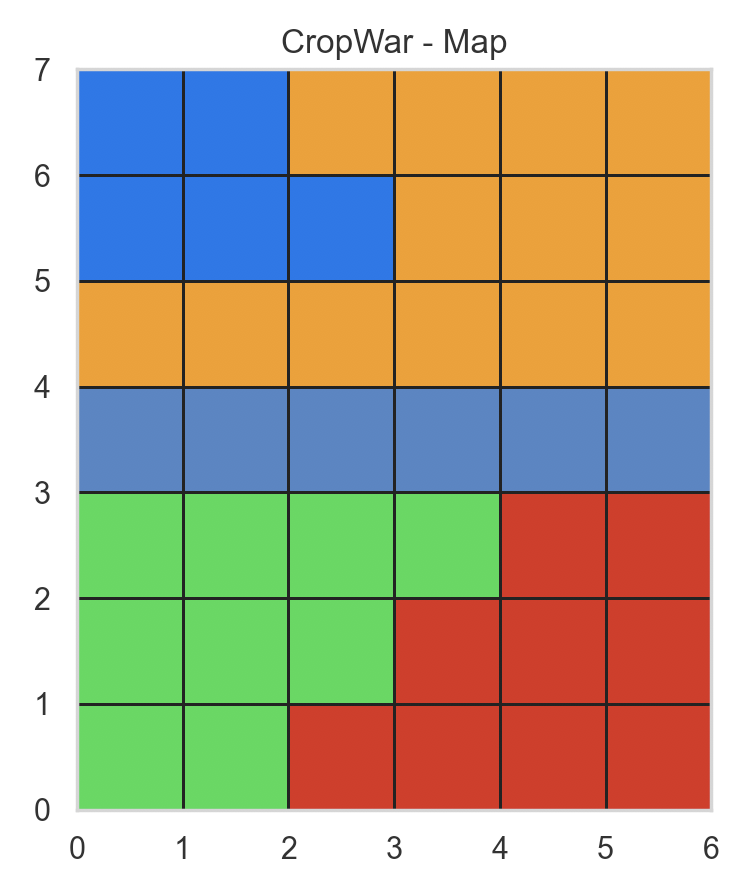
\includegraphics[width=.8\textwidth]{Figures/v12_Map_50t.png}
     \end{figure}
    \column{0.52\linewidth}
    If we extend the simulation to 50 time steps, all available land is bought by farmers
  \end{columns}
\end{frame}

\begin{frame}{\aa}{\aab}
  \begin{columns}
    \column{0.48\linewidth}
    \resizebox{\linewidth}{!}{\begin{tikzpicture}
      \pgfplotsset{
        scale only axis,
      }
      %axis options:
      \begin{axis}[
        xlabel=Time step (years),
        ylabel=Farmer land count (cells),
        xmin=0,
        legend pos=north west,
        cycle list name=farmerslist
      ]
        %plot 1: farmer ID 1
        \addplot+[] 
          table[y index =1]{\cellcountc};
        \addlegendentry{$1$}
        
        %plot 2: farmer ID 2
        \addplot+[]  table[y index =2]{\cellcountc};
        \addlegendentry{$2$}
    
        %plot 3: farmer ID 3
        \addplot+[] table[y index =3]{\cellcountc};
        \addlegendentry{$3$}
    
        %plot 4: farmer ID 4
        \addplot+[] table[y index =4]{\cellcountc};
        \addlegendentry{$4$}
    
      \end{axis}
      \end{tikzpicture}
    }
    \column{0.52\linewidth}
    \resizebox{\linewidth}{!}{\begin{tikzpicture}
      \pgfplotsset{
        scale only axis,
      }
      
      \begin{axis}[
        xlabel=Time step (years),
        ylabel=Farmer stock,
        xmin=0,
        ymin=0,
        legend pos=north west,
        cycle list name=farmerslist
      ]
        %plot 1: farmer ID 1
      \addplot+[dashed] table[y index =5]{\stockc};
      \addlegendentry{$1$}
      
      %plot 2: farmer ID 2
      \addplot+[]  table[y index =2]{\stockc};
      \addlegendentry{$2$}
  
      %plot 3: farmer ID 3
      \addplot+[] table[y index =3]{\stockc};
      \addlegendentry{$3$}
  
      %plot 4: farmer ID 4
      \addplot+[] table[y index =4]{\stockc};
      \addlegendentry{$4$}
  
      \end{axis}
      \end{tikzpicture}
    }
  \end{columns}
\end{frame}

\begin{frame}{\aa}{\aab}
  \begin{columns}
    \column{0.48\linewidth}
    \centering
    \begin{figure}
      \resizebox{\linewidth}{!}{\begin{tikzpicture}
        \pgfplotsset{
          scale only axis,
        }
        %axis options:
        \begin{axis}[
          xlabel=Time step (years),
          ylabel=Farmer wealth (\$),
          xmin=0,
          legend pos=north west,
          cycle list name=farmerslist
        ]
          %plot 1: farmer ID 1
          \addplot+[] 
            table[y index =1]{\budgetc};
          \addlegendentry{$1$}
          
          %plot 2: farmer ID 2
          \addplot+[]  table[y index =2]{\budgetc};
          \addlegendentry{$2$}
      
          %plot 3: farmer ID 3
          \addplot+[] table[y index =3]{\budgetc};
          \addlegendentry{$3$}
      
          %plot 4: farmer ID 4
          \addplot+[] table[y index =4]{\budgetc};
          \addlegendentry{$4$}
      
        \end{axis}
        \end{tikzpicture}
        }
     \end{figure}
    \column{0.52\linewidth}
    On the long run, farmers with more land become wealthier, although the type of crop also seems to have an importance
  \end{columns}
\end{frame}

\begin{frame}{\aa}{\aac}
  \centering
  \textbf{v1.3: Dynamic pricing of crops}
\end{frame}

\begin{frame}{\aa}{\aac}
 \onslide<1->{In \tagg{v1.3} we implement a \texttt{Market} class, which updates the price of crops based on supply and demand.}\\
 \begin{enumerate}
    \item<2-> Harvesting period: agents harvest according to their crop choice and add the harvest yield to the stock. 
    \item<3->Interaction period: market interaction takes place.
    \item<4-> Strategy period: the trader type of the farmers will react on market prices and eventually change the crop.
\end{enumerate}
\end{frame}

\begin{frame}{\aa}{\aac}
    Supply and demand are calculated as follows for a price $p_j$ of crop $j$ grown by farmer $i$:\\
    \begin{equation}
      S_i(p_j) = A + c_i \cdot p_j
    \end{equation}
  Here $c_i$ is the willingness to supply crop $j$  at a given price $p_j$ by farmer $i$ and $A$ is the surplus or his willingness to supply crops for free.
  \begin{equation}
    D_j(p_j) = \left( D_0 + at^2 \right) e^{-\alpha (p_j-p_{j0})}
  \end{equation}
Where $D_0$ is a base demand, $at^2$ is a term representing population (and demand) growth as a function of time $t$, $p_j$ is the price of crop $j$ at time $t$, $p_{j,0}$ is the base price of crop $j$, and $\alpha$ is a demand slope, representing the fact that less and less people will be able to afford expensive crops.
\end{frame}

\pgfplotstableread[col sep=comma]{Data/v13_exported_budget.csv}{\budgetc}
\pgfplotstableread[col sep=comma, skip first n=3]{Data/v13_exported_stock.csv}{\stockc}
\pgfplotstableread[col sep=comma, skip first n=1]{Data/v13_exported_cellcount.csv}{\cellcountc}
\pgfplotstableread[col sep=comma]{Data/v13_exported_demand.csv}{\demandc}
\pgfplotstableread[col sep=comma]{Data/v13_exported_prices.csv}{\pricesc}
\pgfplotstableread[col sep=comma]{Data/v13_exported_supply.csv}{\supplyc}
\pgfplotstableread[col sep=comma]{Data/v13_exported_global_stock.csv}{\globalstockc}


\begin{frame}{\aa}{\aac}
  \begin{columns}
    \column{0.5\linewidth}
    \resizebox{\linewidth}{!}{\begin{tikzpicture}
		\pgfplotsset{
			scale only axis,
		}
		%axis options:
		\begin{axis}[
		  xlabel=Time step (years),
		  ylabel=Demand for different crops,
		  xmin=0,
		  xmax=30,
		  legend pos=south east,
		  cycle list name=cropslist
		]
		  %plot 1: farmer ID 1
		  \addplot+[] 
			  table[y index =1]{\demandc};
		  \addlegendentry{$1$}
		  
		  %plot 2: farmer ID 2
		  \addplot+[]  table[y index =2]{\demandc};
		  \addlegendentry{$2$}
  
		  %plot 3: farmer ID 3
		  \addplot+[] table[y index =3]{\demandc};
		  \addlegendentry{$3$}
  
		  %plot 4: farmer ID 4
		  \addplot+[] table[y index =4]{\demandc};
		  \addlegendentry{$4$}
  
		\end{axis}
	  \end{tikzpicture}
	}
    \column{0.5\linewidth}
    \resizebox{\linewidth}{!}{\begin{tikzpicture}
		\pgfplotsset{
			scale only axis,
		}
		%axis options:
		\begin{axis}[
		  xlabel=Time step (years),
		  ylabel=Supply for different crops,
		  xmin=0,
		  xmax=30,
		  legend pos=south east,
		  cycle list name=cropslist
		]
		  %plot 1: farmer ID 1
		  \addplot+[] 
			  table[y index =1]{\supplyc};
		  \addlegendentry{$1$}
		  
		  %plot 2: farmer ID 2
		  \addplot+[]  table[y index =2]{\supplyc};
		  \addlegendentry{$2$}
  
		  %plot 3: farmer ID 3
		  \addplot+[] table[y index =3]{\supplyc};
		  \addlegendentry{$3$}
  
		  %plot 4: farmer ID 4
		  \addplot+[] table[y index =4]{\supplyc};
		  \addlegendentry{$4$}
  
		\end{axis}
	  \end{tikzpicture}
	  }
  \end{columns}
\end{frame}

\begin{frame}{\aa}{\aac}
\begin{columns}
    \column{0.5\linewidth}
    \resizebox{\linewidth}{!}{\begin{tikzpicture}
		\pgfplotsset{
			scale only axis,
		}
	  
		\begin{axis}[
		  xlabel=Time step (years),
		  ylabel=Prices of different crops,
		  xmin=0,
		  ymin=0,
		  legend pos=north west,
		  cycle list name=cropslist
		]
		  %plot 1: farmer ID 1
	  \addplot+[] table[y index =1]{\pricesc};
	  \addlegendentry{$1$}
	  
	  %plot 2: farmer ID 2
	  \addplot+[]  table[y index =2]{\pricesc};
	  \addlegendentry{$2$}

	  %plot 3: farmer ID 3
	  \addplot+[] table[y index =3]{\pricesc};
	  \addlegendentry{$3$}

	  %plot 4: farmer ID 4
	  \addplot+[] table[y index =4]{\pricesc};
	  \addlegendentry{$4$}

	  \end{axis}
	  \end{tikzpicture}
  }
    \column{0.5\linewidth}
    \resizebox{\linewidth}{!}{\begin{tikzpicture}
		\pgfplotsset{
			scale only axis,
		}
	  
		\begin{axis}[
		  xlabel=Time step (years),
		  ylabel=Total stock of different crops,
		  xmin=0,
		  ymin=0,
		  legend pos=north west,
		  cycle list name=cropslist
		]

		  \addplot+[] table[y index =1]{\globalstockc};
		  \addlegendentry{$1$}
		  \addplot+[] table[y index =2]{\globalstockc};
		  \addlegendentry{$2$}
		  \addplot+[] table[y index =3]{\globalstockc};
		  \addlegendentry{$3$}
		  \addplot+[] table[y index =4]{\globalstockc};
		  \addlegendentry{$4$}
		\end{axis}
	  \end{tikzpicture}
  }
  \end{columns}
\end{frame}

\begin{frame}{\aa}{\aac}
\begin{columns}
    \column{0.45\linewidth}
    \resizebox{\linewidth}{!}{
		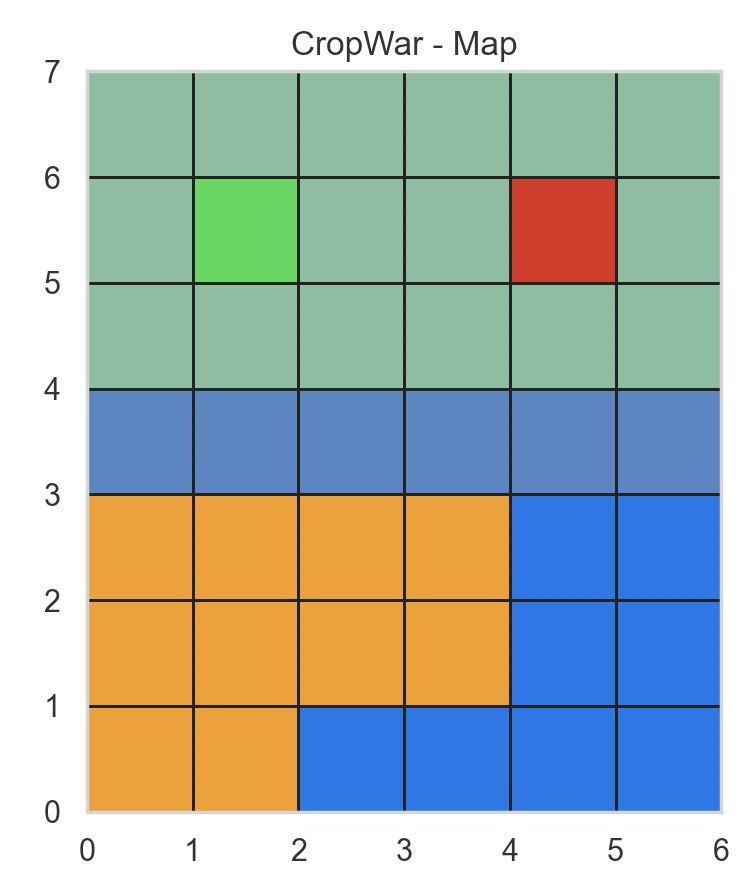
\includegraphics[width=\textwidth]{Figures/v13_Map.png}
	}
    \column{0.5\linewidth}
    \resizebox{\linewidth}{!}{\begin{tikzpicture}
		\pgfplotsset{
			scale only axis,
		}
		%axis options:
		\begin{axis}[
		  xlabel=Time step (years),
		  ylabel=Farmer wealth (\$),
		  xmin=0,
		  %ymin=350,
		  legend pos=north west,
		  cycle list name=farmerslist
		]
		  %plot 1: farmer ID 1
		  \addplot+[] table[y index =1]{\budgetc};
		  \addlegendentry{$1$}
		  
		  %plot 2: farmer ID 2
		  \addplot+[]  table[y index =2]{\budgetc};
		  \addlegendentry{$2$}
  
		  %plot 3: farmer ID 3
		  \addplot+[] table[y index =3]{\budgetc};
		  \addlegendentry{$3$}
  
		  %plot 4: farmer ID 4
		  \addplot+[] table[y index =4]{\budgetc};
		  \addlegendentry{$4$}
  
		\end{axis}
	  \end{tikzpicture}
	  }
  \end{columns}
\end{frame}

\subsection{\ab}
\subsubsection{\aba}

\begin{frame}{\ab}{\aba}
  \centering
  \textbf{v2.1: Reinforcement Learning}
\end{frame}


\begin{frame}{\ab}{\aba}
  \centering
    \begin{figure}
      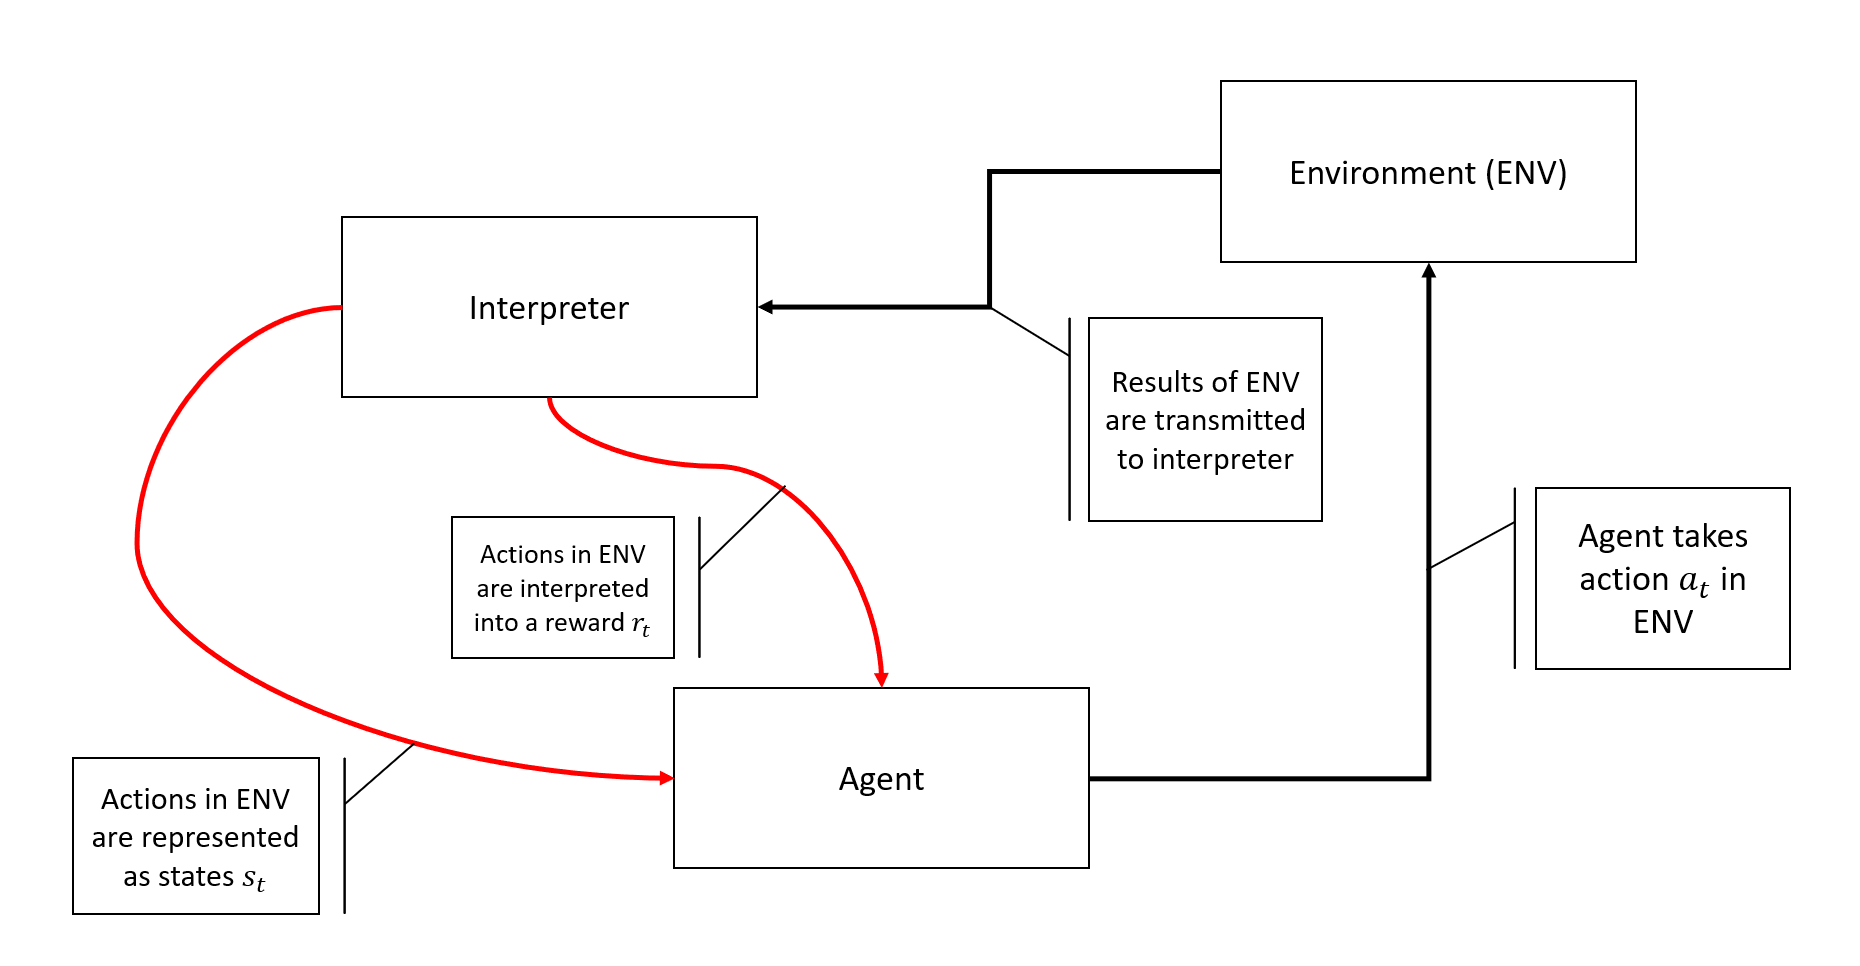
\includegraphics[width = .8\textwidth]{Figures/RL schematic.PNG}
      \caption*{\tiny Feedback loop in RL. An agent decides to do a certain action $a_t$ based on his observation of the environment. This affects the environment, which yields a new state. The effect of the agents' action is then interpreted to update the strategy of the agent.}
    \end{figure}
\end{frame}


\subsubsection{\aac}
\subsubsection{\aad}
\subsubsection{\aae}

\subsection{\ab}


\subsubsection{\abb}

%-------------------------------------------------------
\section{\b}
%-------------------------------------------------------

%%%%%%%%%%%%%%%%%%%%%%%%%%%%%%%%


\begin{frame}{Crop war in perspectives}{FAO-based crop model}{}

  \begin{figure}
   \hfill
        \newline 
     \centering
     \begin{subfigure}[b]{0.45\textwidth}

         \centering
         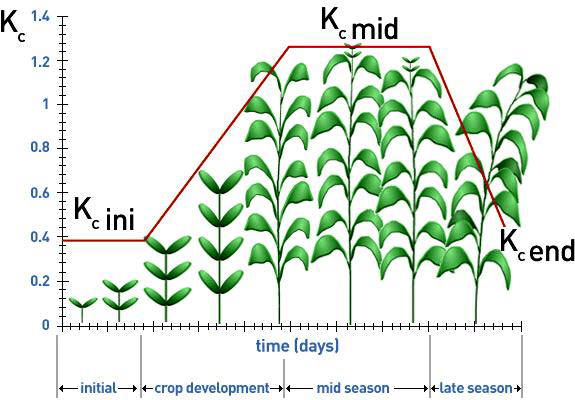
\includegraphics[width=\textwidth]{Figures/Crop-coefficients-Kc-and-growing-period-of-tomato-source-Allen-et-al-1998.png}
         \label{fig:y equals x}
     \end{subfigure}
 \hfill
     \begin{subfigure}[b]{0.45\textwidth}
         \centering
         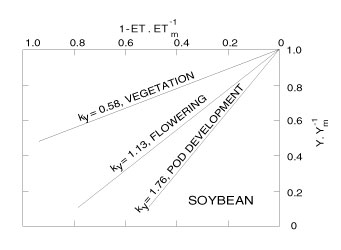
\includegraphics[width=\linewidth]{Figures/Y3655E01.jpeg}
     \end{subfigure}
     \hfill

\end{figure}
 
    \begin{equation}
            1-\frac{Y_t^c}{Y^{m.c}}=\sum_{i=1}^{n} k_{y.i} \cdot(1-\frac{ET_{a.t}^c}{ET_{m.i}}) 
    \end{equation}

\end{frame}

\begin{frame}{Crop war in perspectives}{Global warming potential (GWP)}{}

\begin{figure}
   \hfill
        \newline 
     \centering
     \begin{subfigure}[b]{0.40\textwidth}

         \centering
         \includegraphics[width=\textwidth]{Figures/Emissions-by-sector-–-pie-charts.png}
     \end{subfigure}
 \hfill
     \begin{subfigure}[b]{0.50\textwidth}
         \centering
         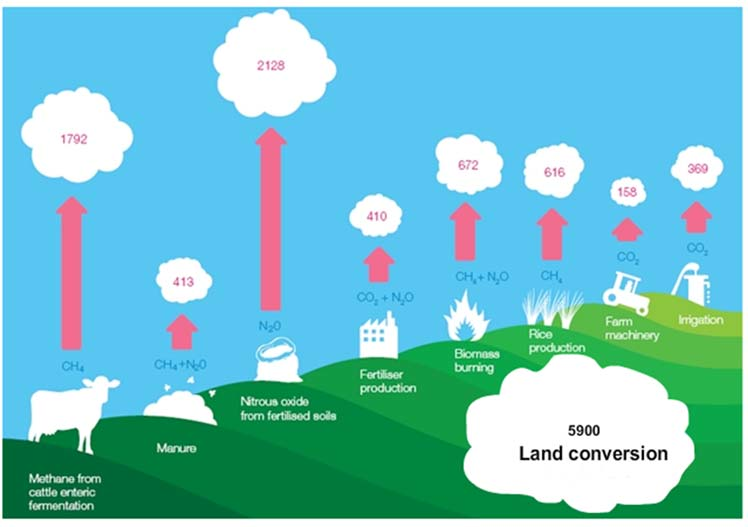
\includegraphics[width=\linewidth]{Figures/GHG-emissions-from-agricultural-sector-by-practices-in-Mt-CO2-e.png}
     \end{subfigure}
     \hfill
     
    \begin{equation}
    GWP_{t}=GWP_{fertilizer}+GWP_{biocide}+GWP_{machinery}+GWP_{electricity}  
    \end{equation}

\end{figure}
 

\end{frame}

\subsubsection{\aac}
\subsubsection{\aad}
\subsubsection{\aae}

\subsection{\ab}


\subsubsection{\abb}
\end{document}

